\subsubsection{UC19 - Visualizzazione avviso: credito insufficiente}
\begin{figure}[H]
	\centering
	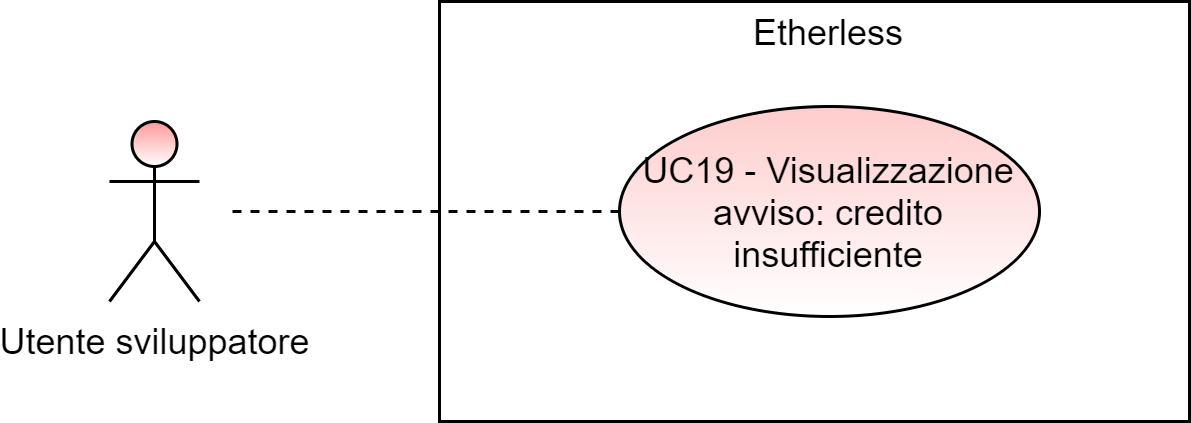
\includegraphics[scale=\ucs]{./res/img/UC19G.png}
	\caption {UC19 - Visualizzazione avviso: credito insufficiente - schema generale}
\end{figure}
\begin{itemize}
	\item \textbf{Attori primari:} \ua{};
	\item \textbf{Attori secondari:} \re{};
	\item \textbf{Descrizione:} l’utente richiede di eseguire un’operazione non avendo abbastanza credito a disposizione. Il sistema riporta un messaggio di errore relativo alla mancanza di credito; 
	\item \textbf{Scenario principale:} viene visualizzato un messaggio di errore relativo alla mancanza di credito necessario per portare a termine l’operazione;
	\item \textbf{Precondizione:} l’utente ha tentato di eseguire un’operazione a pagamento non avendo abbastanza credito a disposizione;  
	\item \textbf{Postcondizione:} la CLI riporta un messaggio di errore. 
\end{itemize}